% AI-GENERATED
% Model  : Claude Opus 4.7
% Date   : 2026-05-19
% Prompt : write tikviz to draw radar graph for intro as paper figure;
%          axes = different degradation levels, hue = datasets.
%          Real numbers only — no hallucinated results.
%
% Data source: paper/egpaper_final.tex
%   - Gaussian noise   : Table tab:gaussian   (mIoU vs clean baseline)
%   - Spatial flips    : Table tab:flips      (flip-back mIoU)
%   - Text degradation : Table tab:text       (mIoU vs clean baseline)
%
% Build:    pdflatex intro_radar.tex
% Include:  
\includegraphics[width=\linewidth]{figs/intro_radar.pdf}

\documentclass[tikz,border=4pt]{standalone}
\usepackage{tikz}

% Click2Act canonical palette (CLAUDE.md Rule 4).
\definecolor{c2aPrimary}{HTML}{2E86AB}    % SA-1B
\definecolor{c2aSecondary}{HTML}{A23B72}  % SACo-Gold
\definecolor{c2aNeutral}{HTML}{6C757D}    % grid / spokes
\definecolor{c2aText}{HTML}{212529}       % labels
\definecolor{c2aBg}{HTML}{F8F9FA}         % figure background

\begin{document}
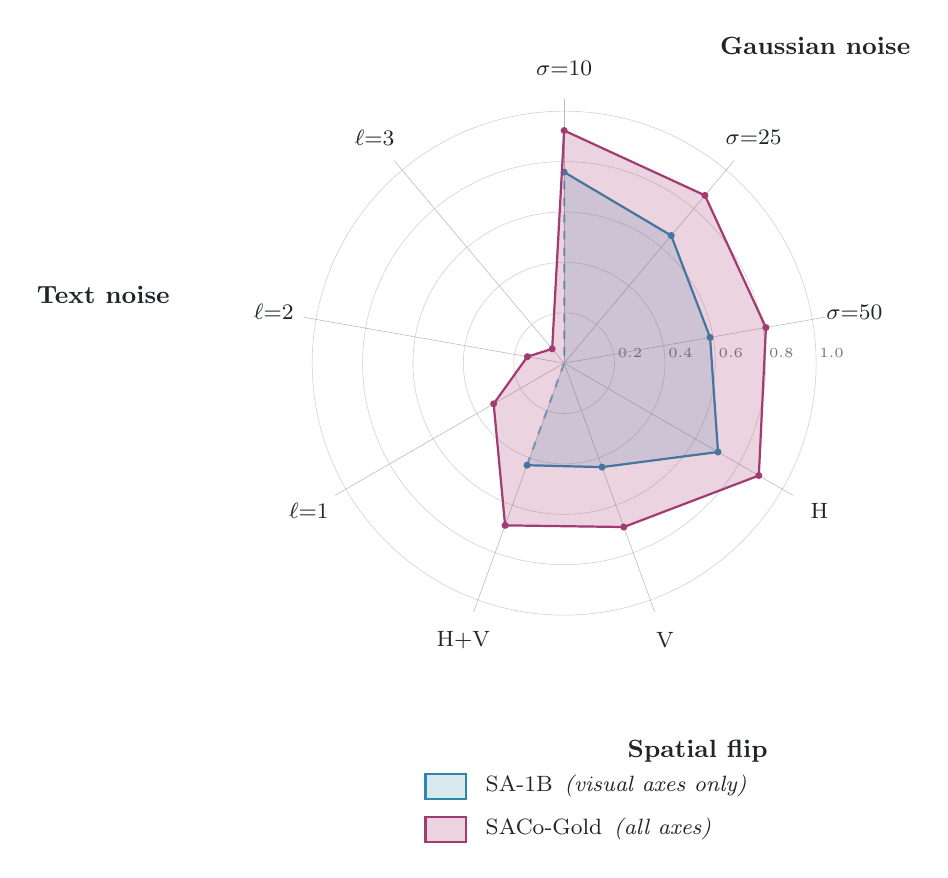
\begin{tikzpicture}[
    scale=3.2,
    every node/.style={font=\small, color=c2aText},
]

% ----------------------------------------------------------------------
% Axis layout (9 spokes, clockwise from top, 40 deg apart)
%   1: Gauss sigma=10        4: Flip H            7: Text l=1
%   2: Gauss sigma=25        5: Flip V            8: Text l=2
%   3: Gauss sigma=50        6: Flip H+V          9: Text l=3
% Angles (degrees):
%   1: 90    2: 50    3: 10    4: -30   5: -70
%   6: -110  7: -150  8: -190  9: -230
% ----------------------------------------------------------------------

% REFINED [old]: filled background panel → [new]: removed per user request (transparent background)
% Concentric reference rings (mIoU = 0.2, 0.4, 0.6, 0.8, 1.0)
\foreach \r in {0.2,0.4,0.6,0.8,1.0}
    \draw[c2aNeutral!35, very thin] (0,0) circle (\r);

% Ring scale on the upward spoke
\foreach \r in {0.2,0.4,0.6,0.8,1.0}
    \node[c2aNeutral, font=\tiny, anchor=west, inner sep=1pt]
        at (\r,0.04) {\r};

% Spokes + per-axis labels
\foreach \ang/\lbl in {
    90/{$\sigma{=}10$},
    50/{$\sigma{=}25$},
    10/{$\sigma{=}50$},
    -30/{H},
    -70/{V},
    -110/{H{+}V},
    -150/{$\ell{=}1$},
    -190/{$\ell{=}2$},
    -230/{$\ell{=}3$}
} {
    \draw[c2aNeutral!50, very thin] (0,0) -- (\ang:1.05);
    \node[anchor=center, font=\footnotesize] at (\ang:1.17) {\lbl};
}

% Category labels (one per degradation family). Anchored so the text grows
% AWAY from the centre, leaving the on-axis labels (sigma=25, V, l=2) clear.
% REFINED [old]: at (50:1.42) {Gaussian noise} → [new]: anchored south, radius 1.55
\node[c2aText, font=\small\bfseries, anchor=south]
    at (50:1.55) {Gaussian noise};
% REFINED [old]: at (-70:1.42) {Spatial flip} → [new]: anchored north, radius 1.55
\node[c2aText, font=\small\bfseries, anchor=north]
    at (-70:1.55) {Spatial flip};
% REFINED [old]: at (-190:1.42) {Text noise} → [new]: anchored east, radius 1.55 (avoids overlap with l=2)
\node[c2aText, font=\small\bfseries, anchor=east]
    at (-190:1.55) {Text noise};

% ----------------------------------------------------------------------
% SA-1B polygon
%   Gaussian mIoU         : 0.758 / 0.661 / 0.588   (Table tab:gaussian)
%   Flip-back mIoU H/V/H+V: 0.705 / 0.439 / 0.431   (Table tab:flips)
%   Text axes             : not applicable (fixed generic prompt)
% Polygon dips to the origin on the text side and the closing chord is
% drawn dashed so the unmeasured sector reads as "n/a", not "zero".
% ----------------------------------------------------------------------
\coordinate (sa1) at ( 90:0.758);
\coordinate (sa2) at ( 50:0.661);
\coordinate (sa3) at ( 10:0.588);
\coordinate (sa4) at (-30:0.705);
\coordinate (sa5) at (-70:0.439);
\coordinate (sa6) at (-110:0.431);
\coordinate (sa0) at (0,0);

\fill[c2aPrimary, opacity=0.18]
    (sa1) -- (sa2) -- (sa3) -- (sa4) -- (sa5) -- (sa6) -- (sa0) -- cycle;
\draw[c2aPrimary, thick]
    (sa1) -- (sa2) -- (sa3) -- (sa4) -- (sa5) -- (sa6);
\draw[c2aPrimary, thick, dashed, opacity=0.55]
    (sa6) -- (sa0) -- (sa1);
\foreach \p in {sa1,sa2,sa3,sa4,sa5,sa6}
    \fill[c2aPrimary] (\p) circle (0.014);

% ----------------------------------------------------------------------
% SACo-Gold polygon
%   Gaussian mIoU         : 0.923 / 0.869 / 0.813   (Table tab:gaussian)
%   Flip-back mIoU H/V/H+V: 0.892 / 0.692 / 0.685   (Table tab:flips)
%   Text mIoU l=1/2/3     : 0.323 / 0.148 / 0.074   (Table tab:text)
% ----------------------------------------------------------------------
\coordinate (sc1) at ( 90:0.923);
\coordinate (sc2) at ( 50:0.869);
\coordinate (sc3) at ( 10:0.813);
\coordinate (sc4) at (-30:0.892);
\coordinate (sc5) at (-70:0.692);
\coordinate (sc6) at (-110:0.685);
\coordinate (sc7) at (-150:0.323);
\coordinate (sc8) at (-190:0.148);
\coordinate (sc9) at (-230:0.074);

\fill[c2aSecondary, opacity=0.22]
    (sc1) -- (sc2) -- (sc3) -- (sc4) -- (sc5)
        -- (sc6) -- (sc7) -- (sc8) -- (sc9) -- cycle;
\draw[c2aSecondary, thick]
    (sc1) -- (sc2) -- (sc3) -- (sc4) -- (sc5)
        -- (sc6) -- (sc7) -- (sc8) -- (sc9) -- cycle;
\foreach \p in {sc1,sc2,sc3,sc4,sc5,sc6,sc7,sc8,sc9}
    \fill[c2aSecondary] (\p) circle (0.014);

% REFINED [old]: SA-1B: n/a callout + leader line → [new]: removed per user request

% ----------------------------------------------------------------------
% Legend (below the plot)
% ----------------------------------------------------------------------
\begin{scope}[shift={(-0.55,-1.70)}]
    \fill[c2aPrimary, opacity=0.18] (0,-0.03) rectangle (0.16,0.07);
    \draw[c2aPrimary, thick]       (0,-0.03) rectangle (0.16,0.07);
    \node[anchor=west, font=\footnotesize] at (0.20,0.02)
        {SA-1B \,\textit{(visual axes only)}};

    \fill[c2aSecondary, opacity=0.22] (0,-0.20) rectangle (0.16,-0.10);
    \draw[c2aSecondary, thick]       (0,-0.20) rectangle (0.16,-0.10);
    \node[anchor=west, font=\footnotesize] at (0.20,-0.15)
        {SACo-Gold \,\textit{(all axes)}};
\end{scope}

% REFINED [old]: radial-axis meaning note inside the figure → [new]: removed; moved to \caption{} in the paper

\end{tikzpicture}
\end{document}